\documentclass[12pt]{decar-wsd}
\usepackage{decar-common}
\usepackage{subdepth}
\usepackage{tikz}
\usepackage{xcolor}
\usetikzlibrary{positioning,calc,decorations.pathreplacing}
\usepackage[percent]{overpic}
\captionsetup[figure]{font=small,labelfont=small}
\usepackage{decar-post}

\title{Closed-Loop Koopman Operator Approximation}
\author{Steven Dahdah\textsuperscript{1} and James Richard Forbes\textsuperscript{2}}

\addbibresource{arxiv-v1.bib}

\begin{document}

% Okabe-Ito colours
\definecolor{oiorange}{rgb}{0.90, 0.60, 0.00}
\definecolor{oiskyblue}{rgb}{0.35, 0.70, 0.90}
\definecolor{oibluishgreen}{rgb}{0.00, 0.60, 0.50}
\definecolor{oiyellow}{rgb}{0.95, 0.90, 0.25}
\definecolor{oiblue}{rgb}{0.00, 0.45, 0.70}
\definecolor{oivermillion}{rgb}{0.80, 0.40, 0.00}
\definecolor{oireddishpurple}{rgb}{0.80, 0.60, 0.70}

\tikzstyle{overview} = [
    draw=gray,
    rounded corners=0.1cm,
    line width=1.5pt,
    minimum height=11cm,
    inner sep=0.1cm,
    anchor=north west,
    align=center,
]

\tikzstyle{block} = [
    draw,
    minimum width=2cm,
    minimum height=1.2cm
]

\tikzstyle{sum} = [
    draw,
    circle,
    minimum size=0.6cm,
]

\tikzstyle{diff} = [
    sum,
    label=170:{\small $+$},
    label=260:{\small $-$}
]

\tikzstyle{summ} = [
    sum,
    label=170:{\small $+$},
    label=80:{\small $+$}
]

\newsavebox{\plant}
\begin{lrbox}{\plant}
    \tikzstyle{block} = [
        draw,
        minimum width=2cm,
        minimum height=1.2cm
    ]
    \begin{tikzpicture}
        \node[
        % ] (in) at (0, 0) {$\mbs{\upsilon}_k^{\mathrm{p}}$};
        ] (in) at (0, 0) {};
        \node[
            block,
            right = 3ex of in
        ] (G) {%
            $\mbs{\mc{P}}
            \stackrel{\min}{\sim}
            \bma{c|c}
                \mbf{A}^\mathrm{p} & \mbf{B}^{\mathrm{p}} \\
                \hline % chktex 44
                \mbf{C}^{\mathrm{p}} & \mbf{D}^{\mathrm{p}}
            \ema$
            };
        \draw[-stealth] (in) -- (G);
        \node[
            right = 3ex of G
        % ] (out) {$\mbs{\zeta}_k^\mathrm{p}$};
        ] (out) {};
        \draw[-stealth] (G) -- (out);
    \end{tikzpicture}
\end{lrbox}

\newsavebox{\closedloop}
\begin{lrbox}{\closedloop}
    \tikzstyle{block} = [
        draw,
        minimum width=2cm,
        minimum height=1.2cm
    ]
    \tikzstyle{sum} = [
        draw,
        circle,
        minimum size=0.6cm,
    ]
    \tikzstyle{diff} = [
        sum,
        label=170:{\small $+$},
        label=260:{\small $-$}
    ]
    \begin{tikzpicture}
        % Plant
        \node[
            block
        ] (plant) at (0, 0) {%
            $\mbs{\mc{P}}
            \stackrel{\min}{\sim}
            \bma{c|c}
                {\mbf{A}^\mathrm{p}} & {\mbf{B}^{\mathrm{p}}} \\
                \hline % chktex 44
                \mbf{C}^{\mathrm{p}} & \mbf{D}^{\mathrm{p}}
            \ema$
        };
        % Current controller
        \node[
            block,
            left=3ex of plant,
        ] (cont_i) {%
            $\mbs{\mc{C}}
            \stackrel{\min}{\sim}
            \bma{c|c}
                \mbf{A}^\mathrm{c} & \mbf{B}^{\mathrm{c}} \\
                \hline % chktex 44
                \mbf{C}^{\mathrm{c}} & \mbf{D}^{\mathrm{c}}
            \ema$
        };
        \draw[-stealth] (cont_i) -- (plant)
            node[midway,above] {};
            % node[midway,above] {${\mbf{y}_k^{\mathrm{c}} = \mbs{\upsilon}_k^\mathrm{p}}$};
        % Current difference
        \node[
            diff,
            left = 3ex of cont_i
        ] (diff_i) {};
        \draw[-stealth] (diff_i) -- (cont_i)
            node[near start,above] {};
            % node[near start,above] {$\mbs{\upsilon}_k^{\mathrm{c}}$};
        \draw[-stealth] (plant.east) -| ++(3ex, -8ex) -| (diff_i)
            node[near end, right] {};
        % Current setpoint
        \node[
            left = 3ex of diff_i
        ] (i_bar) {$\mbf{r}_k$};
        \draw[-stealth] (i_bar) -- (diff_i);
        \node[
            right = 6ex of plant,
        ] (out) {};
        % ] (out) {};
        \draw[-stealth] (plant) -- (out);
        % \draw[-stealth] (plant) -- (out) node[midway,above] {$\mbs{\zeta}_k^{\mathrm{p}}$};
        \node[
            % below = 12ex of cont_i,
            below right = 12ex and 0ex of cont_i.south,
        ] (pic2) {%
            \begin{overpic}[width=3cm]{./figures/state_2.pdf}
               \put(-10, -10){\includegraphics[width=3cm]{./figures/state_1.pdf}}
               \put(-20, -20){\includegraphics[width=3cm]{./figures/state_0.pdf}}
            \end{overpic}
        };
        \node[
            % below = 12ex of plant,
            below right = 12ex and 0ex of plant.south,
        ] (pic3) {%
            \begin{overpic}[width=3cm]{./figures/posvel_2.pdf}
               \put(-10, -10){\includegraphics[width=3cm]{./figures/posvel_1.pdf}}
               \put(-20, -20){\includegraphics[width=3cm]{./figures/posvel_0.pdf}}
            \end{overpic}
        };
        % \node at (i_bar |- pic2) (pic1) {%
        \node[
            below right = 13.6ex and 0ex of i_bar.south,
        ] (pic1) {%
            \begin{overpic}[width=3cm]{./figures/ref_2.pdf}
               \put(-10, -10){\includegraphics[width=3cm]{./figures/ref_1.pdf}}
               \put(-20, -20){\includegraphics[width=3cm]{./figures/ref_0.pdf}}
            \end{overpic}
        };
        \node[
            above = 0ex of pic1,
        ] (lab1) {
            \textit{Reference} $\mbf{r}_k$
        };
        \node[
            above = 0ex of pic2,
        ] (lab2) {
            \textit{Controller state} $\mbf{x}_k^{\mathrm{c}}$
        };
        \node[
            above = 0ex of pic3,
        ] (lab3) {
            \textit{Plant state $\mbf{x}_k^{\mathrm{p}}$}
        };
        \draw[
            -latex,
            line width=2pt,
            shorten <= 0ex,
            shorten >= 0ex,
        ] (i_bar) -- (lab1);
        \draw[
            -latex,
            line width=2pt,
            shorten <= 1ex,
            shorten >= 0ex,
        ] (cont_i) -- (lab2);
        \draw[
            -latex,
            line width=2pt,
            shorten <= 1ex,
            shorten >= 0ex,
        ] (plant) -- (lab3);
    \end{tikzpicture}
\end{lrbox}

\maketitle

\begin{abstract}
    \noindent The Koopman operator allows a nonlinear system to be rewritten
    as an infinite-dimensional linear system by viewing it in terms of an
    infinite set of lifting functions instead of a state vector.
    %
    The main feature of this representation is its linearity, making it
    compatible with existing linear systems theory.
    %
    A finite-dimensional approximation of the Koopman operator can be identified
    from experimental data by choosing a finite subset of lifting functions,
    applying it to the data, and solving a least squares problem in the lifted
    space.
    %
    Existing Koopman operator approximation methods are designed to identify
    open-loop systems. However, it is impractical or impossible to run
    experiments on some systems without a feedback controller. Unfortunately,
    the introduction of feedback control results in correlations between the
    system's input and output, making some plant dynamics difficult to identify
    if the controller is neglected.
    %
    This paper addresses this limitation by introducing a method to identify a
    Koopman model of the closed-loop system, and then extract a Koopman model of
    the plant given knowledge of the controller. This is accomplished by
    leveraging the linearity of the Koopman representation of the system. The
    proposed approach widens the applicability of Koopman operator
    identification methods to a broader class of systems.
    %
    The effectiveness of the proposed closed-loop Koopman operator approximation
    method is demonstrated experimentally using a Harmonic Drive gearbox
    exhibiting nonlinear vibrations.
\end{abstract}

\section{Introduction}\label{sec:introduction}

Using Koopman operator theory~\cite{koopman_hamiltonian_1931,
mezic_2019_spectrum, budisic_applied_2012, mauroy_2020_koopman}, a
finite-dimensional nonlinear system can be rewritten as an infinite-dimensional
linear system.
%
The Koopman operator itself serves to advance the infinite-dimensional system's
state in time, much like the dynamics matrix of a linear system.
%
Since, in practice, working with an infinite-dimensional operator is
intractable, the Koopman operator is approximated as a finite-dimensional
matrix, often using data-driven methods.
%
While the Koopman operator was originally proposed almost one hundred years ago,
recent theoretical results~\cite{mezic_2019_spectrum, budisic_applied_2012,
mauroy_2020_koopman} paired with modern computational resources have led to it
becoming a popular tool for identifying dynamical systems from data.

In a typical Koopman workflow, a set of lifting functions is first chosen. In
some situations, these lifting functions are inspired by the dynamics of the
system~\cite{abraham_active_2019, mamakoukas_local_2019}, while in others, they
are taken from a standard set of basis functions, like polynomials, sinusoids,
or radial basis functions~\cite{bruder_modeling_2019, abraham_model-based_2017}.
Lifting functions can also be chosen to approximate a given
kernel~\cite{guo_2022_koopman, degennaro_2019_scalable, rahimi_2007_random}.
Time delays are often incorporated into the lifted state as
well~\cite{korda_2018_linear, bruder_modeling_2019}. Once the chosen lifting
functions are applied to the data, linear regression is used to approximate the
Koopman matrix, often with some form of
regularization~\cite{bruder_modeling_2019}.

One of the key properties of the Koopman operator is its linearity, making it
possible to leverage existing linear systems theory when identifying or
analyzing Koopman systems.
%
Moreover, the linear Koopman representation of the nonlinear system allows
linear control design methods to be leveraged~\cite{korda_2018_linear,
otto_2021_koopman, abraham_active_2019, mamakoukas_local_2019,
bruder_modeling_2019, uchida_2021_data-driven}. Koopman operator approximation
methods are also closely related to classical system identification
methods~\cite{korda_2018_linear}, most notably subspace identification
methods~\cite[\S3]{brunton_2022_modern}.
%
This similarity means that well-established system identification techniques can
often be adapted to enrich the Koopman workflow. One area of particular interest
is the identification of closed-loop systems~\cite{forssell_1999_closedloop,
hof_1998_closedloop, ljung_1999_system}. It is often impossible to run an
experiment on a plant without a feedback control system, either because the
plant is inherently unstable, or because it is unsafe or impractical to do
so~\cite[\S1.1, \S17.3]{ljung_1999_system}. In some cases the control loop is
simply ignored and control outputs are treated as exogenous input signals to the
plant~\cite[\S13.5]{ljung_1999_system}. However, this simplification, known as
the \textit{direct approach}, is not without its issues. The feedback loop
introduces correlations between the plant's output and its input, leading to
biased estimates of the plant's dynamics~\cite[\S11.1]{katayama_2005_subspace}.
In cases where this bias is small, ignoring the control loop may be acceptable.
In cases where the bias is not small, closed-loop system identification methods
must be employed. These methods identify the closed-loop system as a whole,
where the reference signal treated as the exogenous input, and then extract the
plant system for use on its own~\cite[\S11.1]{katayama_2005_subspace}. Methods
that use knowledge of the controller are known as \textit{indirect
approaches}~\cite[\S13.5]{ljung_1999_system}.
%
In contrast, methods that identify an unknown controller along with the plant
are categorized as \textit{joint input-output
approaches}~\cite[\S13.5]{ljung_1999_system}. While closed-loop system
identification can lead to more complex plant models, in many situations it is
the appropriate tool to use to avoid biased models. In some situations,
closed-loop system identification must be used due to the inability to operate
the plant in an open-loop fashion.

\begin{figure}[ht]
    \centering
    \resizebox{\textwidth}{!}{\begin{tikzpicture}
        \node[
            overview,
            minimum width=4.5cm,
            label={north:(a) Collect data snapshots from closed-loop system},
        ] (step1) at (0, 0) {%
            \usebox{\closedloop}\\[5ex]
            \textit{Known:}
            $\mbs{\mc{C}}
            \stackrel{\min}{\sim}
            \bma{c|c}
                \mbf{A}^\mathrm{c} & \mbf{B}^{\mathrm{c}} \\
                \hline % chktex 44
                \mbf{C}^{\mathrm{c}} & \mbf{D}^{\mathrm{c}}
            \ema,\ 
            \mbf{C^\mathrm{p}} = \diag\left\{\mbf{1}, \mbf{0}\right\},\ 
            \mbf{D^\mathrm{p}} = \mbf{0}$ \\[2ex]
            \textit{Unknown:}
            $\mbf{U}^\mathrm{p}
            =
            \begin{bmatrix}
                \mbf{A^{\!\mathrm{p}}} & \mbf{B^\mathrm{p}}
            \end{bmatrix}$
        };
        \node[
            overview,
            right=0.25cm of step1,
            label={north:(b) Identify closed-loop system},
        ] (step2) {%
            \textit{Lifted plant state:}\\[1ex]
            \begin{overpic}[width=3cm]{./figures/lift_2.pdf}
               \put(-10, -10){\includegraphics[width=3cm]{./figures/lift_1.pdf}}
               \put(-20, -20){\includegraphics[width=3cm]{./figures/lift_0.pdf}}
            \end{overpic}\\[3ex]
            \begin{tikzpicture}
                \draw[-latex, line width=2pt] (0cm, 0cm) -- (0cm, -0.8cm);
            \end{tikzpicture}
            \\
            % \textit{Arrange lifted snapshots:}\\[1ex]
            \textit{Extended DMD:}\\[2ex]
            $\mbs{\Psi} = \begin{bmatrix}
                \mbf{x}_0^\mathrm{c} &
                    \mbf{x}_1^\mathrm{c} &
                    \cdots &
                    \mbf{x}_{q-1}^\mathrm{c} \\[1ex]
                \mbs{\vartheta}_0^\mathrm{p} &
                    \mbs{\vartheta}_1^\mathrm{p} &
                    \cdots &
                    \mbs{\vartheta}_{q-1}^\mathrm{p} \\
                \mbf{r}_0 &
                    \mbf{r}_1 &
                    \cdots &
                    \mbf{r}_{q-1}
            \end{bmatrix}$\\[2ex]
            $\mbs{\Theta}_+ = \begin{bmatrix}
                \mbf{x}_1^\mathrm{c} &
                    \mbf{x}_2^\mathrm{c} &
                    \cdots &
                    \mbf{x}_{q}^\mathrm{c} \\[1ex]
                \mbs{\vartheta}_1^\mathrm{p} &
                    \mbs{\vartheta}_2^\mathrm{p} &
                    \cdots &
                    \mbs{\vartheta}_{q}^\mathrm{p}
            \end{bmatrix}$
            \\[2ex]
            % \begin{tikzpicture}
            %     \draw[-latex, line width=2pt] (0cm, 0cm) -- (0cm, -0.8cm);
            % \end{tikzpicture}
            % \\
            % \textit{Extended DMD:}\\
            $\mbf{U}^\mathrm{f} = \arg \underset{\mbf{U}}{\min}\|\mbs{\Theta}_+ - \mbf{U}\mbs{\Psi}\|_\frob^2$
        };
        \node[
            overview,
            right=0.25cm of step2,
            label={north:(c) Recover plant system},
        ] (step4) {%
            \textit{CL Koopman matrix:}\\[1ex]
            $\mbf{U}^{\mathrm{f}}
            =
            \begin{bmatrix}
                \mbf{U}_{11}^{\mathrm{f}} &
                \mbf{U}_{12}^{\mathrm{f}} &
                \mbf{U}_{13}^{\mathrm{f}} \\
                \mbf{U}_{21}^{\mathrm{f}} &
                \mbf{U}_{22}^{\mathrm{f}} &
                \mbf{U}_{23}^{\mathrm{f}}.
            \end{bmatrix}$
            \\[1ex]
            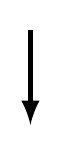
\begin{tikzpicture}
                % \draw[-latex, line width=2pt] (0cm, 0cm) -- (0cm, -0.8cm);
                \draw[-latex, line width=2pt] (0cm, 0cm) -- (0cm, -1.2cm);
            \end{tikzpicture}
            \\
            \textit{Plant Koopman matrix:}\\[1ex]
            $\mbf{A}^{\!\mathrm{p}}
            =
            \mbf{U}_{22}^{\mathrm{f}}
            +
            \mbf{U}_{23}^{\mathrm{f}}
            \mbf{C}^{\mathrm{p}}$
            \\[1ex]
            $\mbf{B}^{\mathrm{p}}
            =
            \begin{bmatrix}
                \mbf{U}_{21}^{\mathrm{f}} &
                \mbf{U}_{23}^{\mathrm{f}}
            \end{bmatrix}
            {\begin{bmatrix}
                \mbf{C}^{\mathrm{c}} &
                \mbf{D}^{\mathrm{c}}
            \end{bmatrix}}^\dagger$
            \\[1ex]
            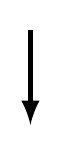
\begin{tikzpicture}
                % \draw[-latex, line width=2pt] (0cm, 0cm) -- (0cm, -0.8cm);
                \draw[-latex, line width=2pt] (0cm, 0cm) -- (0cm, -1.2cm);
            \end{tikzpicture}
            \\
            \textit{Plant Koopman system:}\\[1ex]
            \usebox{\plant}
        };
    \end{tikzpicture}}
    \caption{Overview of the proposed closed-loop Koopman operator
    identification method. To simplify the presentation, no feedforward signal
    is used. (a) First, the controller reference, controller state, and plant
    state are recorded during a series of experiments. The controller state
    space matrices are known, and $\mbf{C}^\mathrm{p}$ and $\mbf{D}^\mathrm{p}$
    are fixed. If the controller state is not directly available, it can be
    computed from its input and output. Only the Koopman matrix of the plant
    $\mbf{U}^\mathrm{p}$ is unknown. (b) The plant state is lifted and augmented
    with the controller state and reference. The Koopman matrix of the
    closed-loop (CL) system, $\mbf{U}^\mathrm{f}$, is approximated. (c) The
    known controller state-space matrices are combined with the identified
    Koopman matrix to compute the Koopman matrix of the plant,
    $\mbf{U}^\mathrm{p}$.}\label{fig:overview}
\end{figure}

The key contribution of this paper is the adaptation of closed-loop system
identification methods to Koopman operator approximation. The proposed method,
summarized in \Cref{fig:overview}, is a variation of the indirect approach,
wherein a Koopman model of the closed-loop system is first identified, and then
the Koopman system modelling the plant is extracted given knowledge of the
controller.
%
The significance of this work is that a system that cannot be operated in
open-loop without a feedback controller can now be identified using Koopman
operator theory.
%
The effectiveness of this method is demonstrated on a motor drive suffering from
nonlinear gearbox vibrations, which would be difficult to identify in an
open-loop setting.

The remainder of this paper is as follows.
%
\Cref{sec:background} outlines the necessary background information on the
Koopman operator and its associated approximation techniques.
%
\Cref{sec:closed_loop} derives the proposed closed-loop Koopman operator
approximation method.
%
\Cref{sec:training} describes the experimental setup used to generate the
motor drive training dataset used in this paper, including the control system
used on the drive.
%
\Cref{sec:design} outlines the important design decisions made in the Koopman
operator approximation procedure, namely the lifting function selection
rationale and the hyperparameter optimization method.
%
\Cref{sec:results} analyzes the experimental results of the closed-loop Koopman
operator approximation method.
%
The paper's conclusions are presented in \Cref{sec:conclusion}.

\section{Background}\label{sec:background}

\subsection{Koopman operator theory}
%
Consider the nonlinear difference equation
\begin{equation}
    \mbf{x}_{k+1} = \mbf{f}(\mbf{x}_{k}),%
    \label{eq:dynamics_no_input}
\end{equation}
where
${\mbf{x}_{k} \in \mc{M}}$
evolves on a manifold
${\mc{M} \subseteq \mathbb{R}^{m \times 1}}$.
%
Also consider an infinite number of scalar-valued \textit{lifting functions},
${\psi: \mc{M} \to \mathbb{R}}$,
which span an infinite-dimensional Hilbert space
$\mc{H}$.
%
The \textit{Koopman operator}, ${\mc{U}: \mc{H} \to \mc{H}}$, is a linear
operator that composes all lifting functions ${\psi \in \mc{H}}$ with
$\mbf{f}(\cdot)$, thereby advancing them in time by
one step. That is~\cite[\S3.2]{kutz_dynamic_2016},
\begin{equation}
    (\mc{U} \psi)(\cdot) = (\psi \circ \mbf{f})(\cdot).%
    \label{eq:koopman_def_no_input}
\end{equation}
%
Evaluating~\cref{eq:koopman_def_no_input} at $\mbf{x}_k$ reveals that the
dynamics of~\cref{eq:dynamics_no_input} can be rewritten linearly in terms of
$\psi$ as
\begin{equation}
    \psi(\mbf{x}_{k+1}) = (\mc{U} \psi)(\mbf{x}_{k}).%
    \label{eq:koopman_dynamics}
\end{equation}
%
A finite-dimensional approximation of~\cref{eq:koopman_dynamics} is
\begin{equation}
    \mbs{\psi}(\mbf{x}_{k+1}) = \mbf{U} \mbs{\psi}(\mbf{x}_{k}) + \mbs{\epsilon}_k,%
    \label{eq:koopman_approx_no_input}
\end{equation}
where
${\mbs{\psi}: \mc{M} \to \mathbb{R}^{p \times 1}}$ is the \textit{vector-valued
    lifting function}, ${\mbf{U} \in \mathbb{R}^{p \times p}}$ is the
\textit{Koopman matrix}, and $\mbs{\epsilon}_k$ is the residual error.

\subsection{Koopman operator theory with inputs}
%
The definition of the Koopman operator can be modified to accommodate nonlinear
difference equations with exogenous inputs. Consider the difference equation
\begin{equation}
    \mbf{x}_{k+1} = \mbf{f}(\mbf{x}_{k}, \mbf{u}_k),\label{eq:dynamics_input}
\end{equation}
where the state is
${\mbf{x}_{k} \in \mc{M} \subseteq \mathbb{R}^{m \times 1}}$
and the input is
${\mbf{u}_{k} \in \mc{N} \subseteq \mathbb{R}^{n \times 1}}$.
%
The lifting functions are now
${\psi: \mc{M} \times \mc{N} \to \mathbb{R}}$
and the Koopman operator
${\mc{U}: \mc{H} \to \mc{H}}$
now satisfies
\begin{equation}
    (\mc{U} \psi)(\mbf{x}_{k}, \mbf{u}_{k})
    = \psi(\mbf{f}(\mbf{x}_{k}, \mbf{u}_k), \star),
    \label{eq:koopman_def_input}
\end{equation}
where
${\star = \mbf{u}_k}$
if the input has state-dependent dynamics, or
${\star = \mbf{0}}$
if the input has no dynamics~\cite[\S6.5]{kutz_dynamic_2016}.
%
Let the vector-valued lifting function
${\mbs{\psi}: \mc{M} \times \mc{N} \to \mathbb{R}^{p \times 1}}$
be partitioned as
\begin{equation}
    \mbs{\psi}(\mbf{x}_k, \mbf{u}_k) = \begin{bmatrix}
        \mbs{\vartheta}(\mbf{x}_k) \\
        \mbs{\upsilon}(\mbf{x}_k, \mbf{u}_k)
    \end{bmatrix},
\end{equation}
where the state-dependent lifting functions are
${\mbs{\vartheta}: \mc{M} \to \mathbb{R}^{p_\vartheta \times 1}}$,
the input-dependent lifting functions are
${\mbs{\upsilon}: \mc{M} \times \mc{N} \to \mathbb{R}^{p_\upsilon \times 1}}$,
and
the lifting function dimensions satisfy
${p_\vartheta + p_\upsilon = p}$.
%
With an exogenous input, substituting the state and input
into~\cref{eq:koopman_def_input} results in~\cite[\S6.5.1]{kutz_dynamic_2016}
\begin{equation}
    \mbs{\vartheta}(\mbf{x}_{k+1}) \\
    =
    \mbf{U}
    \mbs{\psi}(\mbf{x}_{k}, \mbf{u}_{k})
    + \mbs{\epsilon}_k,%
    \label{eq:U_part}
\end{equation}
where ${\mbf{U} = \begin{bmatrix} \mbf{A} & \mbf{B} \end{bmatrix}}$.
Expanding~\cref{eq:U_part} yields the familiar linear state-space form,
\begin{equation}
    \mbs{\vartheta}(\mbf{x}_{k+1})
    =
    \mbf{A} \mbs{\vartheta}(\mbf{x}_{k})
    + \mbf{B} \mbs{\upsilon}(\mbf{x}_k, \mbf{u}_k)
    + \mbs{\epsilon}_k.
\end{equation}

When designing lifting functions, the first $m$ lifted states are often chosen
to be the state of the original difference equation,
$\mbf{x}_k$. Specifically,~\cite[\S3.3.1]{kutz_dynamic_2016}
\begin{equation}
    \mbs{\vartheta}(\mbf{x}_k)
    =
    \begin{bmatrix}
        \mbf{x}_k \\
        \vartheta_m(\mbf{x}_k) \\
        \vartheta_{m + 1}(\mbf{x}_k) \\
        \vdots \\
        \vartheta_{p_\vartheta - 1}(\mbf{x}_k)
    \end{bmatrix}.
\end{equation}
This choice of lifting functions makes it easier to recover the original state
from the lifted state.
%
Another common design decision is to leave the input unlifted when identifying
a Koopman model for control. That is~\cite{korda_2018_linear},
\begin{equation}
    \mbs{\upsilon}(\mbf{x}_k, \mbf{u}_k) = \mbf{u}_k.
\end{equation}
However, recent work has also shown that bilinear input-dependent lifting
functions are a better alternative for control affine
systems~\cite{bruder_2021_advantages}.

An output equation,
\begin{equation}
    \mbs{\zeta}_k = \mbf{C} \mbs{\vartheta}_k + \mbf{D} \mbs{\upsilon}_k,
\end{equation}
where $\mbs{\zeta}_k \in \mathbb{R}^{p_\zeta \times 1}$,
can also be considered to incorporate the Koopman operator into a true linear
system with input, output, and state. While $\mbf{D} = \mbf{0}$ in all cases,
$\mbf{C}$ can be chosen to recover the original states, or any other desired
output.
%
If the original state is not directly included in the lifted state, $\mbf{C}$
can instead be determined using least squares~\cite[\S3.2.1]{korda_2018_linear}.
The \textit{Koopman system} is therefore
\begin{equation}
    \mbs{\mc{G}}
    \stackrel{\min}{\sim}
    \bma{c|c}
        \mbf{A} & \mbf{B} \\
        \hline % chktex 44
        \mbf{C} & \mbf{D}
    \ema,
\end{equation}
where $\stackrel{\min}{\sim}$ denotes a minimal state space
realization~\cite[\S3.2.1]{green_linear_1994}.


\subsection{Approximating the Koopman operator from data}
%
To approximate the Koopman matrix from a dataset
${\mc{D} = {\{\mbf{x}_k, \mbf{u}_k\}}_{k=0}^q}$,
consider the lifted snapshot matrices
\begin{align}
    \mbs{\Psi} &= \begin{bmatrix}
        \mbs{\psi}_{0} & \mbs{\psi}_{1} & \cdots & \mbs{\psi}_{q-1}
    \end{bmatrix} \in \mathbb{R}^{p \times q}, \\
    \mbs{\Theta}_+ &= \begin{bmatrix}
        \mbs{\vartheta}_{1} & \mbs{\vartheta}_{2} & \cdots & \mbs{\vartheta}_{q}
    \end{bmatrix} \in \mathbb{R}^{p_\vartheta \times q},\label{eq:Theta}
\end{align}
where
${\mbs{\psi}_k = \mbs{\psi}(\mbf{x}_k, \mbf{u}_k)}$
and
${\mbs{\vartheta}_k = \mbs{\vartheta}(\mbf{x}_k)}$.
%
The Koopman matrix that minimizes
\begin{equation}
    J(\mbf{U}) = \|\mbs{\Theta}_+ - \mbf{U} \mbs{\Psi}\|_\frob^2
\end{equation}
is~\cite[\S1.2.1]{kutz_dynamic_2016}
\begin{equation}
    \mbf{U} = \mbs{\Theta}_+ \mbs{\Psi}^\dagger,
\end{equation}
where ${(\cdot)}^\dagger$ denotes the Moore-Penrose pseudoinverse.

Often, Tikhonov regularization is included to improve the numerical conditioning
of $\mbf{U}$ by penalizing its squared Frobenius
norm~\cite{tikhonov_1995_numerical}. The cost function then becomes
\begin{equation}
     J(\mbf{U}) = \|\mbs{\Theta}_+ - \mbf{U} \mbs{\Psi}\|_\frob^2
     + \beta \|\mbf{U}\|_\frob^2,
 \end{equation}
where $\beta$ is the regularization coefficient.

\section{Closed-loop approximation of the Koopman operator}\label{sec:closed_loop}

In this section the proposed closed-loop Koopman operator approximation method
is outlined in detail. First, the Koopman representation of the closed-loop
system is derived in terms of the known state-space matrices of the controller
and the unknown Koopman matrix of the plant. Then, a method for extracting the
unknown plant Koopman matrix from the identified closed-loop system is
described. This method is inspired by the joint-input output subspace
identification method of~\cite[\S11.2.2]{katayama_2005_subspace}.
%
However, since the state-space matrices of the controller are required to
recover the plant model, it is closer to an indirect system identification
approach.

\subsection{Formulating the closed-loop Koopman system}

Consider the Koopman system modelling the plant,
\begin{align}
    \mbs{\vartheta}_{k+1}^{\mathrm{p}}
    &=
    \mbf{A}^{\!\mathrm{p}}
    \mbs{\vartheta}_{k}^{\mathrm{p}}
    +
    \mbf{B}^{\mathrm{p}}
    \mbs{\upsilon}_{k}^{\mathrm{p}},
    \\
    \mbs{\zeta}_{k}^{\mathrm{p}}
    &=
    \mbf{C}^{\mathrm{p}}
    \mbs{\vartheta}_{k}^{\mathrm{p}}
    +
    \mbf{D}^{\mathrm{p}}
    \mbs{\upsilon}_{k}^{\mathrm{p}},
\end{align}
along with the linear system modelling the known controller,
\begin{align}
    \mbf{x}_{k+1}^{\mathrm{c}}
    &=
    \mbf{A}^{\!\mathrm{c}}
    \mbf{x}_{k}^{\mathrm{c}}
    +
    \mbf{B}^{\mathrm{c}}
    \mbf{u}_{k}^{\mathrm{c}},
    \\
    \mbf{y}_{k}^{\mathrm{c}}
    &=
    \mbf{C}^{\mathrm{c}}
    \mbf{x}_{k}^{\mathrm{c}}
    +
    \mbf{D}^{\mathrm{c}}
    \mbf{u}_{k}^{\mathrm{c}}.
\end{align}
In the Koopman system, only $\mbf{A}^{\!\mathrm{p}}$ and $\mbf{B}^{\mathrm{p}}$
are determined from experimental data. The remaining state-space matrices are
chosen to be
\begin{align}
    \mbf{C}^{\mathrm{p}}
    &=
    \begin{bmatrix}
        \mbf{1}_{m \times m} & \mbf{0}_{m \times (p_{\vartheta} - m)}
    \end{bmatrix},\label{eq:C_def}
    \\
    \mbf{D}^{\mathrm{p}}
    &=
    \mbf{0},\label{eq:D_def}
\end{align}
such that $\mbf{C}^{\mathrm{p}}$ recovers the original states of the nonlinear
system being modelled, which are the first $m$ states in
$\mbs{\vartheta}_k^\mathrm{p}$.

Let
\begin{equation}
    \mbs{\upsilon}_{k}^{\mathrm{p}}
    =
    \mbf{y}_{k}^{\mathrm{c}}
    +
    \mbf{f}_{k},
\end{equation}
which yields the series interconnection of the controller and the plant with
a feedforward signal $\mbf{f}_k$.
%
This feedforward signal is entirely exogenous, and could be generated by a
nonlinear inverse model of the plant.
%
The new Koopman system's input includes the controller input and feedforward
input, resulting in
\begin{equation}
    \mbs{\upsilon}_{k}^{\mathrm{s}}
    =
    \begin{bmatrix}
        \mbf{u}_{k}^{\mathrm{c}} \\
        \mbf{f}_{k}
    \end{bmatrix},\label{eq:upsilon_s}
\end{equation}
while its output is simply the plant output,
${\mbs{\zeta}_{k} = \mbs{\zeta}_{k}^{\mathrm{p}}}$.
The new system's state includes the controller state and plant state, resulting
in
\begin{equation}
    \mbs{\vartheta}_k
    =
    \begin{bmatrix}
        \mbf{x}_{k}^{\mathrm{c}} \\
        \mbs{\vartheta}_{k}^{\mathrm{p}}
    \end{bmatrix}.
\end{equation}
The cascaded plant and controller systems are depicted
in \Cref{fig:series_interconnection}.
%
\begin{figure}[htb]
    \centering
    \begin{tikzpicture}
        \node[
        ] (in) at (0, 0) {$\mbf{u}_k^{\mathrm{c}}$};

        \node[
            above = 6ex of in
        ] (ff) at (0, 0) {$\mbf{f}_k$};

        \draw[
            decorate,
            decoration = {brace},
            line width = 1pt,
        ] ([xshift=-2ex]in.south) -- ([xshift=-2ex]ff.north)
        node[
            midway, left
        ] {$\mbs{\upsilon}_k^{\mathrm{s}}=$};

        \node[
            block,
            right = 6ex of in
        ] (G) {$\mbs{\mc{C}}$};
        \draw[-stealth] (in) -- (G);

        \node[
            summ,
            right = 6ex of G,
        ] (sum) {};

        \node[
            block,
            right = 6ex of sum
        ] (W) {$\mbs{\mc{P}}$};

        \node[
            right = 6ex of W
        ] (out) {$\mbs{\zeta}_k^\mathrm{p} = \mbs{\zeta}_k$};

        \draw[-stealth] (G) -- (sum)
            node[midway, above] {$\mbf{y}_k^{\mathrm{c}}$};
        \draw[-stealth] (sum) -- (W)
            node[midway, above] {$\mbs{\upsilon}_k^{\mathrm{p}}$};
        \draw[-stealth] (ff) -| (sum);
        \draw[-stealth] (W) -- (out);
    \end{tikzpicture}
    \caption{Series interconnection of the controller and
    plant.}\label{fig:series_interconnection}
\end{figure}

The state space representation of the plant becomes
\begin{align}
    \mbs{\vartheta}_{k+1}^{\mathrm{p}}
    &=
    \mbf{A}^{\!\mathrm{p}}
    \mbs{\vartheta}_{k}^{\mathrm{p}}
    +
    \mbf{B}^{\mathrm{p}}
    \left(
        \mbf{C}^{\mathrm{c}}
        \mbf{x}_{k}^{\mathrm{c}}
        +
        \mbf{D}^{\mathrm{c}}
        \mbf{u}_{k}^{\mathrm{c}}
        +
        \mbf{f}_k
    \right)
    \\
    &=
    \begin{bmatrix}
        \mbf{B}^{\mathrm{p}} \mbf{C}^{\mathrm{c}} &
        \mbf{A}^{\!\mathrm{p}}
    \end{bmatrix}
    \begin{bmatrix}
        \mbf{x}_{k}^{\mathrm{c}} \\
        \mbs{\vartheta}_{k}^{\mathrm{p}}
    \end{bmatrix}
    +
    \begin{bmatrix}
        \mbf{B}^{\mathrm{p}}
        \mbf{D}^{\mathrm{c}}
        &
        \mbf{B}^{\mathrm{p}}
    \end{bmatrix}
    \begin{bmatrix}
        \mbf{u}_{k}^{\mathrm{c}} \\
        \mbf{f}_k
    \end{bmatrix},
    \\
    \mbs{\zeta}_{k}^{\mathrm{p}}
    &=
    \mbf{C}^{\mathrm{p}}
    \mbs{\vartheta}_{k}^{\mathrm{p}}
    +
    \mbf{D}^{\mathrm{p}}
    \left(
        \mbf{C}^{\mathrm{c}}
        \mbf{x}_{k}^{\mathrm{c}}
        +
        \mbf{D}^{\mathrm{c}}
        \mbf{u}_{k}^{\mathrm{c}}
        +
        \mbf{f}_k
    \right)
    \\
    &=
    \begin{bmatrix}
        \mbf{D}^{\mathrm{p}} \mbf{C}^{\mathrm{c}} &
        \mbf{C}^{\mathrm{p}}
    \end{bmatrix}
    \begin{bmatrix}
        \mbf{x}_{k}^{\mathrm{c}} \\
        \mbs{\vartheta}_{k}^{\mathrm{p}}
    \end{bmatrix}
    +
    \begin{bmatrix}
        \mbf{D}^{\mathrm{p}}
        \mbf{D}^{\mathrm{c}}
        &
        \mbf{D}^{\mathrm{p}}
    \end{bmatrix}
    \begin{bmatrix}
        \mbf{u}_{k}^{\mathrm{c}} \\
        \mbf{f}_k
    \end{bmatrix}.
\end{align}
The state space representation of the series-interconnected system is therefore
\begin{align}
    \begin{bmatrix}
        \mbf{x}_{k+1}^{\mathrm{c}} \\
        \mbs{\vartheta}_{k+1}^{\mathrm{p}}
    \end{bmatrix}
    &=
    \begin{bmatrix}
        \mbf{A}^{\!\mathrm{c}} &
        \mbf{0} \\
        \mbf{B}^{\mathrm{p}} \mbf{C}^{\mathrm{c}} &
        \mbf{A}^{\!\mathrm{p}}
    \end{bmatrix}
    \begin{bmatrix}
        \mbf{x}_{k}^{\mathrm{c}} \\
        \mbs{\vartheta}_{k}^{\mathrm{p}}
    \end{bmatrix}
    +
    \begin{bmatrix}
        \mbf{B}^{\mathrm{c}}
        &
        \mbf{0}
        \\
        \mbf{B}^{\mathrm{p}}
        \mbf{D}^{\mathrm{c}}
        &
        \mbf{B}^{\mathrm{p}}
    \end{bmatrix}
    \begin{bmatrix}
        \mbf{u}_{k}^{\mathrm{c}}\\
        \mbf{f}_{k}
    \end{bmatrix},
    \\
    \mbs{\zeta}_{k}^{\mathrm{p}}
    &=
    \begin{bmatrix}
        \mbf{D}^{\mathrm{p}} \mbf{C}^{\mathrm{c}} &
        \mbf{C}^{\mathrm{p}}
    \end{bmatrix}
    \begin{bmatrix}
        \mbf{x}_{k}^{\mathrm{c}} \\
        \mbs{\vartheta}_{k}^{\mathrm{p}}
    \end{bmatrix}
    +
    \begin{bmatrix}
        \mbf{D}^{\mathrm{p}}
        \mbf{D}^{\mathrm{c}}
        &
        \mbf{D}^{\mathrm{p}}
    \end{bmatrix}
    \begin{bmatrix}
        \mbf{u}_{k}^{\mathrm{c}}\\
        \mbf{f}_{k}
    \end{bmatrix},
\end{align}
or equivalently,
\begin{align}
    \mbs{\vartheta}_{k+1}
    &=
    \begin{bmatrix}
        \mbf{A}^{\!\mathrm{c}} &
        \mbf{0} \\
        \mbf{B}^{\mathrm{p}} \mbf{C}^{\mathrm{c}} &
        \mbf{A}^{\!\mathrm{p}}
    \end{bmatrix}
    \mbs{\vartheta}_{k}
    +
    \begin{bmatrix}
        \mbf{B}^{\mathrm{c}}
        &
        \mbf{0}
        \\
        \mbf{B}^{\mathrm{p}}
        \mbf{D}^{\mathrm{c}}
        &
        \mbf{B}^{\mathrm{p}}
    \end{bmatrix}
    \mbs{\upsilon}_{k}^{\mathrm{s}},\label{eq:open_loop_state}
    \\
    \mbs{\zeta}_{k}
    &=
    \begin{bmatrix}
        \mbf{D}^{\mathrm{p}} \mbf{C}^{\mathrm{c}} &
        \mbf{C}^{\mathrm{p}}
    \end{bmatrix}
    \mbs{\vartheta}_{k}
    +
    \begin{bmatrix}
        \mbf{D}^{\mathrm{p}}
        \mbf{D}^{\mathrm{c}}
        &
        \mbf{D}^{\mathrm{p}}
    \end{bmatrix}
    \mbs{\upsilon}_{k}^{\mathrm{s}}.\label{eq:open_loop_output}
\end{align}

Next, consider the negative feedback interconnection,
\begin{equation}
    \mbf{u}_k^{\mathrm{c}}
    =
    \mbf{r}_k
    -
    \mbs{\zeta}_k,\label{eq:feedback_u}
\end{equation}
where $\mbf{r}_k$ is an exogenous reference signal. The input of
this new feedback-interconnected system is defined to be
\begin{equation}
    \mbs{\upsilon}_k
    =
    \begin{bmatrix}
        \mbf{r}_k \\
        \mbf{f}_k
    \end{bmatrix},
\end{equation}
as depicted in \Cref{fig:feedback_interconnection}.
Substituting~\cref{eq:feedback_u} into~\cref{eq:upsilon_s}
yields
\begin{align}
    \mbs{\upsilon}_{k}^{\mathrm{s}}
    &=
    \begin{bmatrix}
        \mbf{r}_k - \mbs{\zeta}_k \\
        \mbf{f}_{k}
    \end{bmatrix}\label{eq:feedback_feedforward}
    \\
    &=
    \mbs{\upsilon}_{k}
    -
    \begin{bmatrix}
        \mbs{\zeta}_k \\
        \mbf{0}
    \end{bmatrix}.
    \label{eq:feedback}
\end{align}

\begin{figure}[htb]
    \centering
    \begin{tikzpicture}

        % Plant
        \node[
            block
        ] (plant) at (0, 0) {$\mbs{\mc{P}}$};

        \node[
            summ,
            left = 4ex of plant,
        ] (sum) {};

        % Current controller
        \node[
            block,
            left=4ex of sum,
        ] (cont_i) {$\mbs{\mc{C}}$};

        \draw[-stealth] (cont_i) -- (sum);

        \draw[-stealth] (sum) -- (plant);

        % Current difference
        \node[
            diff,
            left = 4ex of cont_i
        ] (diff_i) {};
        \draw[-stealth] (diff_i) -- (cont_i)
            node[midway,above] {$\mbf{u}_k^{\mathrm{c}}$};
        \draw[-stealth] (plant.east) -| ++(4ex, -8ex) -| (diff_i)
            node[near end, right]{$\mbs{\zeta}_k$};

        % Current setpoint
        \node[
            left = 4ex of diff_i
        ] (i_bar) {$\mbf{r}_k$};

        \draw[-stealth] (i_bar) -- (diff_i);

        \node[
            above = 4ex of i_bar
        ] (ff) {$\mbf{f}_k$};

        \draw[-stealth] (ff) -| (sum);

        \draw[
            decorate,
            decoration = {brace},
            line width = 1pt,
        ] ([xshift=-2ex]i_bar.south) -- ([xshift=-2ex]ff.north)
        node[
            midway, left
        ] {$\mbs{\upsilon}_k=$};

        \node[
            right = 8ex of plant,
        ] (out) {$\mbs{\zeta}_k$};
        \draw[-stealth] (plant) -- (out);

    \end{tikzpicture}
    \caption{Feedback interconnection of the controller and
    plant.}\label{fig:feedback_interconnection}
\end{figure}

Substituting~\cref{eq:feedback} into~\cref{eq:open_loop_output} results in a
new output equation,
\begin{align}
    \mbs{\zeta}_{k}
    &=
    \begin{bmatrix}
        \mbf{D}^{\mathrm{p}} \mbf{C}^{\mathrm{c}} &
        \mbf{C}^{\mathrm{p}}
    \end{bmatrix}
    \mbs{\vartheta}_{k}
    +
    \begin{bmatrix}
        \mbf{D}^{\mathrm{p}}
        \mbf{D}^{\mathrm{c}} &
        \mbf{D}^{\mathrm{p}}
    \end{bmatrix}
    \mbs{\upsilon}_k
    -
    \begin{bmatrix}
        \mbf{D}^{\mathrm{p}}
        \mbf{D}^{\mathrm{c}} &
        \mbf{D}^{\mathrm{p}}
    \end{bmatrix}
    \begin{bmatrix}
        \mbs{\zeta}_{k} \\
        \mbf{0}
    \end{bmatrix}
    \\
    &=
    {\left(
        \mbf{1}
        +
        \mbf{D}^{\mathrm{p}}
        \mbf{D}^{\mathrm{c}}
    \right)}^{-1}
    \begin{bmatrix}
        \mbf{D}^{\mathrm{p}} \mbf{C}^{\mathrm{c}} &
        \mbf{C}^{\mathrm{p}}
    \end{bmatrix}
    \mbs{\vartheta}_{k}
    +
    {\left(
        \mbf{1}
        +
        \mbf{D}^{\mathrm{p}}
        \mbf{D}^{\mathrm{c}}
    \right)}^{-1}
    \begin{bmatrix}
        \mbf{D}^{\mathrm{p}}
        \mbf{D}^{\mathrm{c}} &
        \mbf{D}^{\mathrm{p}}
    \end{bmatrix}
    \mbs{\upsilon}_k,\label{eq:feedback_output}
\end{align}
where the feedback interconnection is \textit{well-posed} if and only if
${\mbf{1} + \mbf{D}^{\mathrm{p}} \mbf{D}^{\mathrm{c}}}$ is
invertible~\cite[\S4.9.1]{skogestad_2006_multivariable}.
%
Let ${\mbf{Q} = \mbf{1} + \mbf{D}^{\mathrm{p}} \mbf{D}^{\mathrm{c}}}$.
%
Substituting~\cref{eq:feedback_output}
into~\cref{eq:feedback} yields
\begin{align}
    \mbs{\upsilon}_k^{\mathrm{s}}
    &=
    \mbs{\upsilon}_k
    -
    \begin{bmatrix}
        {\mbf{Q}}^{-1}
        \mbf{D}^{\mathrm{p}} \mbf{C}^{\mathrm{c}} &
        {\mbf{Q}}^{-1}
        \mbf{C}^{\mathrm{p}} \\
        \mbf{0} &
        \mbf{0}
    \end{bmatrix}
    \mbs{\vartheta}_{k}
    -
    \begin{bmatrix}
        {\mbf{Q}}^{-1}
        \mbf{D}^{\mathrm{p}}
        \mbf{D}^{\mathrm{c}} &
        {\mbf{Q}}^{-1}
        \mbf{D}^{\mathrm{p}} \\
        \mbf{0} &
        \mbf{0}
    \end{bmatrix}
    \mbs{\upsilon}_k
    \\
    &=
    \begin{bmatrix}
        -
        {\mbf{Q}}^{-1}
        \mbf{D}^{\mathrm{p}} \mbf{C}^{\mathrm{c}} &
        -
        {\mbf{Q}}^{-1}
        \mbf{C}^{\mathrm{p}} \\
        \mbf{0} &
        \mbf{0}
    \end{bmatrix}
    \mbs{\vartheta}_{k}
    +
    \begin{bmatrix}
        \mbf{1}
        -
        {\mbf{Q}}^{-1}
        \mbf{D}^{\mathrm{p}}
        \mbf{D}^{\mathrm{c}} &
        -
        {\mbf{Q}}^{-1}
        \mbf{D}^{\mathrm{p}} \\
        \mbf{0} &
        \mbf{1}
    \end{bmatrix}
    \mbs{\upsilon}_k.\label{eq:feedback_input}
\end{align}
Substituting~\cref{eq:feedback_input} back into~\cref{eq:open_loop_state}
results in a new state equation,
\begin{multline}
    \mbs{\vartheta}_{k+1}
    =
    \left(
        \begin{bmatrix}
            \mbf{A}^{\!\mathrm{c}} &
            \mbf{0} \\
            \mbf{B}^{\mathrm{p}} \mbf{C}^{\mathrm{c}} &
            \mbf{A}^{\!\mathrm{p}}
        \end{bmatrix}
        +
        \begin{bmatrix}
            \mbf{B}^{\mathrm{c}} &
            \mbf{0}
            \\
            \mbf{B}^{\mathrm{p}}
            \mbf{D}^{\mathrm{c}} &
            \mbf{B}^{\mathrm{p}}
        \end{bmatrix}
        \begin{bmatrix}
            -
            {\mbf{Q}}^{-1}
            \mbf{D}^{\mathrm{p}} \mbf{C}^{\mathrm{c}} &
            -
            {\mbf{Q}}^{-1}
            \mbf{C}^{\mathrm{p}} \\
            \mbf{0} &
            \mbf{0}
        \end{bmatrix}
    \right)
    \mbs{\vartheta}_{k}
    \\
    +
    \begin{bmatrix}
        \mbf{B}^{\mathrm{c}} &
        \mbf{0}
        \\
        \mbf{B}^{\mathrm{p}}
        \mbf{D}^{\mathrm{c}} &
        \mbf{B}^{\mathrm{p}}
    \end{bmatrix}
    \begin{bmatrix}
        \mbf{1}
        -
        {\mbf{Q}}^{-1}
        \mbf{D}^{\mathrm{p}}
        \mbf{D}^{\mathrm{c}} &
        -
        {\mbf{Q}}^{-1}
        \mbf{D}^{\mathrm{p}} \\
        \mbf{0} &
        \mbf{1}
    \end{bmatrix}
    \mbs{\upsilon}_{k}.
\end{multline}
Rearranging yields the state-space representation of the closed-loop system,
with the state equation being
\begin{multline}
    \mbs{\vartheta}_{k+1}
    =
    \begin{bmatrix}
        \mbf{A}^{\mathrm{c}}
            - \mbf{B}^{\mathrm{c}}
            {\mbf{Q}}^{-1}
            \mbf{D}^{\mathrm{p}}\mbf{C}^{\mathrm{c}}
            &
        - \mbf{B}^{\mathrm{c}}
            {\mbf{Q}}^{-1}
            \mbf{C}^{\mathrm{p}}
            \\
        \mbf{B}^{\mathrm{p}} \mbf{C}^{\mathrm{c}}
            - \mbf{B}^{\mathrm{p}} \mbf{D}^{\mathrm{c}}
            {\mbf{Q}}^{-1}
            \mbf{D}^{\mathrm{p}}\mbf{C}^{\mathrm{c}}
            &
        \mbf{A}^{\mathrm{p}}
            - \mbf{B}^{\mathrm{p}} \mbf{D}^{\mathrm{c}}
            {\mbf{Q}}^{-1}
            \mbf{C}^{\mathrm{p}}
            \\
    \end{bmatrix}
    \mbs{\vartheta}_{k}
    \\
    +
    \begin{bmatrix}
        \mbf{B}^{\mathrm{c}} - \mbf{B}^{\mathrm{c}}
            {\mbf{Q}}^{-1}
            \mbf{D}^{\mathrm{p}}
            \mbf{D}^{\mathrm{c}}
        &
        -
        \mbf{B}^{\mathrm{c}}
        {\mbf{Q}}^{-1}
        \mbf{D}^{\mathrm{p}}
        \\
        \mbf{B}^{\mathrm{p}} \mbf{D}^{\mathrm{c}}
            - \mbf{B}^{\mathrm{p}} \mbf{D}^{\mathrm{c}}
            {\mbf{Q}}^{-1}
            \mbf{D}^{\mathrm{p}}
            \mbf{D}^{\mathrm{c}}
        &
        \mbf{B}^{\mathrm{p}}
        -
        \mbf{B}^{\mathrm{p}}
        \mbf{D}^{\mathrm{c}}
        {\mbf{Q}}^{-1}
        \mbf{D}^{\mathrm{p}}
    \end{bmatrix}
    \mbs{\upsilon}_{k},
\end{multline}
and the output equation being
\begin{equation}
    \mbs{\zeta}_{k}
    =
    \begin{bmatrix}
        {\mbf{Q}}^{-1}
        \mbf{D}^{\mathrm{p}} \mbf{C}^{\mathrm{c}} &
        {\mbf{Q}}^{-1}
        \mbf{C}^{\mathrm{p}}
    \end{bmatrix}
    \mbs{\vartheta}_{k}
    +
    \begin{bmatrix}
        {\mbf{Q}}^{-1}
        \mbf{D}^{\mathrm{p}}
        \mbf{D}^{\mathrm{c}} &
        {\mbf{Q}}^{-1}
        \mbf{D}^{\mathrm{p}}
    \end{bmatrix}
    \mbs{\upsilon}_k.
\end{equation}
Substituting in ${\mbf{D}^\mathrm{p} = \mbf{0}}$ from~\cref{eq:D_def} implies
that ${\mbf{Q} = \mbf{1}}$ and yields the simplified state-space
representation,
\begin{align}
    \mbs{\vartheta}_{k+1}
    &=
    \underbrace{%
        \begin{bmatrix}
            \mbf{A}^{\mathrm{c}} &
            - \mbf{B}^{\mathrm{c}} \mbf{C}^{\mathrm{p}} \\
            \mbf{B}^{\mathrm{p}} \mbf{C}^{\mathrm{c}} &
            \mbf{A}^{\mathrm{p}} - \mbf{B}^{\mathrm{p}} \mbf{D}^{\mathrm{c}} \mbf{C}^{\mathrm{p}} \\
        \end{bmatrix}
    }_{\mbf{A}^{\!\mathrm{f}}}
    \mbs{\vartheta}_{k}
    +
    \underbrace{%
        \begin{bmatrix}
            \mbf{B}^{\mathrm{c}}
            &
            \mbf{0}
            \\
            \mbf{B}^{\mathrm{p}} \mbf{D}^{\mathrm{c}}
            &
            \mbf{B}^{\mathrm{p}}
        \end{bmatrix}
    }_{\mbf{B}^\mathrm{f}}
    \mbs{\upsilon}_{k},
    \\
    \mbs{\zeta}_{k}
    &=
    \underbrace{%
        \begin{bmatrix}
            \mbf{0} &
            \mbf{C}^{\mathrm{p}}
        \end{bmatrix}
    }_{\mbf{C}^\mathrm{f}}
    \mbs{\vartheta}_{k}
    +
    \underbrace{%
        \mbf{0}
    }_{\mbf{D}^\mathrm{f}}
    \,
    \mbs{\upsilon}_{k},
\end{align}
which is always a well-posed feedback interconnection, since
${\mbf{Q} = \mbf{1} + \mbf{D}^{\mathrm{p}} \mbf{D}^{\mathrm{c}} = \mbf{1}}$.

\subsection{Extracting the plant Koopman system}

Consider the closed-loop lifted dataset
${\mathcal{D} = {\left\{\mbs{\vartheta}_k, \mbs{\upsilon}_k\right\}}_{k=0}^q}$,
where the matrix approximation of the Koopman operator is
\begin{align}
    \mbf{U}^{\mathrm{f}}
    &=
    \begin{bmatrix}
        \mbf{A}^{\!\mathrm{f}} &
        \mbf{B}^{\mathrm{f}}
    \end{bmatrix}
    \\
    &=
    \begin{bmatrix}
        \mbf{A}^{\mathrm{c}} &
        - \mbf{B}^{\mathrm{c}} \mbf{C}^{\mathrm{p}} &
        \mbf{B}^{\mathrm{c}} &
        \mbf{0}
        \\
        \mbf{B}^{\mathrm{p}} \mbf{C}^{\mathrm{c}} &
        \mbf{A}^{\mathrm{p}} - \mbf{B}^{\mathrm{p}} \mbf{D}^{\mathrm{c}} \mbf{C}^{\mathrm{p}} &
        \mbf{B}^{\mathrm{p}} \mbf{D}^{\mathrm{c}} &
        \mbf{B}^{\mathrm{p}}
    \end{bmatrix}
    \\
    &=
    \begin{bmatrix}
        \mbf{U}_{11}^{\mathrm{f}} &
        \mbf{U}_{12}^{\mathrm{f}} &
        \mbf{U}_{13}^{\mathrm{f}} &
        \mbf{U}_{14}^{\mathrm{f}} \\
        \mbf{U}_{21}^{\mathrm{f}} &
        \mbf{U}_{22}^{\mathrm{f}} &
        \mbf{U}_{23}^{\mathrm{f}} &
        \mbf{U}_{24}^{\mathrm{f}}
    \end{bmatrix}.\label{eq:Uf}
\end{align}
Since $\mbf{C}^{\mathrm{p}}$ is known,
$\mbf{A}^{\!\mathrm{p}}$ can be
recovered using
$\mbf{U}_{22}^{\mathrm{f}}$ and $\mbf{U}_{23}^{\mathrm{f}}$ with
\begin{equation}
    \mbf{A}^{\!\mathrm{p}}
    =
    \mbf{U}_{22}^{\mathrm{f}}
    +
    \mbf{U}_{23}^{\mathrm{f}}
    \mbf{C}^{\mathrm{p}}.\label{eq:A_p}
\end{equation}
Similarly, $\mbf{B}^\mathrm{p}$, $\mbf{U}_{21}^{\mathrm{f}}$,
$\mbf{U}_{23}^{\mathrm{f}}$, and $\mbf{U}_{24}^{\mathrm{f}}$ are
related via the expression
\begin{equation}
    \mbf{B}^{\mathrm{p}}
    {\begin{bmatrix}
        \mbf{C}^{\mathrm{c}} &
        \mbf{D}^{\mathrm{c}} &
        \mbf{1}
    \end{bmatrix}}
    =
    \begin{bmatrix}
        \mbf{U}_{21}^{\mathrm{f}} &
        \mbf{U}_{23}^{\mathrm{f}} &
        \mbf{U}_{24}^{\mathrm{f}}
    \end{bmatrix}.
\end{equation}
As a result, $\mbf{B}^{\mathrm{p}}$ can be recovered with
\begin{equation}
    \mbf{B}^{\mathrm{p}}
    =
    \begin{bmatrix}
        \mbf{U}_{21}^{\mathrm{f}} &
        \mbf{U}_{23}^{\mathrm{f}} &
        \mbf{U}_{24}^{\mathrm{f}}
    \end{bmatrix}
    {\begin{bmatrix}
        \mbf{C}^{\mathrm{c}} &
        \mbf{D}^{\mathrm{c}} &
        \mbf{1}
    \end{bmatrix}}^\dagger,\label{eq:B_p}
\end{equation}
where ${(\cdot)}^\dagger$ denotes the Moore-Penrose pseudoinverse.

\section{Training setup}\label{sec:training}

\begin{figure}[ht]
    \centering
    \includegraphics[width=0.5\linewidth]{drive.jpg}
    \caption{Motor drive used to generate the training data, which consists of a
    motor with Harmonic Drive gearbox. The gearbox introduces nonlinear
    oscillations into the system, leading to tracking errors at specific
    frequencies.}\label{fig:test_bench}
\end{figure}

The advantages of the proposed closed-loop Koopman operator approximation method
are demonstrated using an experimental dataset gathered from a motor drive with
Harmonic Drive gearbox. The motor drive, pictured in \Cref{fig:test_bench},
exhibits nonlinear vibrations due to the dynamics of the gearbox.
%
Since it is not practical or safe to operate such a motor drive in open-loop, it
is operated using a simple linear position and velocity controller.
%
This section describes how the dataset was collected and details the control
system used to run the experiments. The sections that follow show that a linear
model of the closed-loop system is unable to identify the nonlinear gearbox
vibrations, while a Koopman model of the closed-loop system is able to model
them.

\subsection{Dataset}

\begin{figure}[htbp]
    \centering
    \includegraphics[width=0.75\linewidth]{./figures/cl_input.pdf}
    \caption{Reference input to the closed-loop drive system from the first test
    episode. The velocity reference is a slightly smoothed pseudorandom binary
    sequence. It was generated by setting pseudorandom position checkpoints at
    the maximum allowable velocity and acceleration in the drive's control
    software.}\label{fig:cl_input}
\end{figure}

The complete motor drive dataset consists of 18 training episodes and 2 test
episodes.
%
The reference position, reference velocity, measured position, measured
velocity, and measured torque are recorded at \SI{1}{\kilo\hertz}.
%
The positions
and velocities are recorded in \si{\radian} and \si{\radian/\second}
respectively at the output shaft of the gearbox, while the measured torque is
recorded as a fraction of the drive's full-scale torque.

\Cref{fig:cl_input} shows a portion of one of the test inputs used to
characterize the closed-loop system.
%
The drive's control software accepts position checkpoints, and generates
smoothed trapezoidal velocity trajectories to reach them.
%
Each episode contains 10 pseudorandom position checkpoints within one revolution
of the gearbox output shaft in either direction. The resulting velocity profile
resembles a smoothed pseudorandom binary sequence. For all episodes, the
maximum allowed velocity and acceleration settings are selected in the drive's
control software.

\subsection{Controller}

The drive's motor controller consists of an inner proportional-integral velocity
loop paired with an outer proportional position loop. While the controller gains
are known, its state-space matrices must be derived for later use in the
closed-loop Koopman operator approximation procedure.

The controller can be represented by the multi-input single-output differential
equation,
\begin{equation}
    \tau(s)
    =
    \left(
    K_\mathrm{p}^{\dot{\theta}}
    +
    \frac{1}{s}
    K_\mathrm{i}^{\dot{\theta}}
    \right)
    \left(
    \dot{\theta}^{\mathrm{e}}(s)
    +
    \vphantom{\frac{1}{s}}  % Force parenthesis size to be consistent
    K_\mathrm{p}^{\theta}
    \,
    \theta^{\mathrm{e}}(s)
    \right),\label{eq:motor_controller}
\end{equation}
where
$\dot{\theta}^{\mathrm{e}}(s) = \dot{\theta}^{\mathrm{r}}(s) - \dot{\theta}(s)$
is the velocity error,
$\theta^{\mathrm{e}}(s) = \theta^{\mathrm{r}}(s) - \theta(s)$
is the position error,
$\dot{\theta}^{\mathrm{r}}(s)$ is the velocity reference,
$\theta^{\mathrm{r}}(s)$ is the position reference,
$\dot{\theta}(s)$ is the motor velocity,
$\theta(s)$ is the motor position,
and $\tau(s)$ is the motor torque.  % TODO Define Laplace variable?
The velocity controller gains are $K_\mathrm{p}^{\dot{\theta}}$ and
$K_\mathrm{i}^{\dot{\theta}}$, while the position controller
gain is $K_\mathrm{p}^{\theta}$.

Discretizing~\cref{eq:motor_controller} using the forward Euler approximation,
where  % TODO Cite Euler approx?
\begin{equation}
    \frac{1}{s}
    =
    \frac{\Delta t}{1 - z^{-1}}
\end{equation}
and $\Delta t$ is the timestep, yields
\begin{align}
    \tau(z)
    &=
    \left(
        K_\mathrm{p}^{\dot{\theta}}
        +
        \frac{\Delta t}{1 - z^{-1}}
        K_\mathrm{i}^{\dot{\theta}}
    \right)
    \left(
        \dot{\theta}^{\mathrm{e}}(z)
        +
        \vphantom{\frac{\Delta t}{1 - z^{-1}}}  % Force parenthesis size
        K_\mathrm{p}^{\theta}
        \,
        \theta^{\mathrm{e}}(z)
    \right)
    \\
    &=
    z^{-1}
    \tau(z)
    +
    \left(
        K_\mathrm{p}^{\dot{\theta}}
        +
        \Delta t
        K_\mathrm{i}^{\dot{\theta}}
        -
        K_\mathrm{p}^{\dot{\theta}}
        z^{-1}
    \right)
    \dot{\theta}^{\mathrm{e}}(z)
    +
    \left(
        K_\mathrm{p}^{\theta}
        K_\mathrm{p}^{\dot{\theta}}
        +
        \Delta t
        K_\mathrm{p}^{\theta}
        K_\mathrm{i}^{\dot{\theta}}
        -
        K_\mathrm{p}^{\theta}
        K_\mathrm{p}^{\dot{\theta}}
        z^{-1}
    \right)
    \theta^{\mathrm{e}}(z).\label{eq:motor_controller_discrete_freq}
\end{align}
In the time domain,~\cref{eq:motor_controller_discrete_freq} is
\begin{align}
    \tau_k
    &=
    \tau_{k-1}
    +
    \left(
        K_\mathrm{p}^{\dot{\theta}}
        +
        \Delta t
        K_\mathrm{i}^{\dot{\theta}}
    \right)
    \dot{\theta}^{\mathrm{e}}_k
    -
    K_\mathrm{p}^{\dot{\theta}}
    \dot{\theta}^{\mathrm{e}}_{k-1}
    +
    \left(
        K_\mathrm{p}^{\theta}
        K_\mathrm{p}^{\dot{\theta}}
        +
        \Delta t
        K_\mathrm{p}^{\theta}
        K_\mathrm{i}^{\dot{\theta}}
    \right)
    \theta^{\mathrm{e}}_k
    -
    K_\mathrm{p}^{\theta}
    K_\mathrm{p}^{\dot{\theta}}
    \theta^{\mathrm{e}}_{k-1}
    \\
    &=
    \tau_{k-1}
    +
    \begin{bmatrix}
        K_\mathrm{p}^{\theta}
        K_\mathrm{p}^{\dot{\theta}}
        +
        \Delta t
        K_\mathrm{p}^{\theta}
        K_\mathrm{i}^{\dot{\theta}}
        &
        K_\mathrm{p}^{\dot{\theta}}
        +
        \Delta t
        K_\mathrm{i}^{\dot{\theta}}
    \end{bmatrix}
    \begin{bmatrix}
        \theta^{\mathrm{e}}_k \\
        \dot{\theta}^{\mathrm{e}}_k
    \end{bmatrix}
    +
    \begin{bmatrix}
        -K_\mathrm{p}^{\theta} K_\mathrm{p}^{\dot{\theta}} &
        -K_\mathrm{p}^{\dot{\theta}}
    \end{bmatrix}
    \begin{bmatrix}
        \theta^{\mathrm{e}}_{k-1} \\
        \dot{\theta}^{\mathrm{e}}_{k-1}
    \end{bmatrix}.\label{eq:motor_controller_discrete}
\end{align}
To find a state-space representation of~\cref{eq:motor_controller_discrete},
let the controller state be
\begin{equation}
    x_k^{\mathrm{c}}
    =
    \tau_k
    -
    \begin{bmatrix}
        K_\mathrm{p}^{\theta}
        K_\mathrm{p}^{\dot{\theta}}
        +
        \Delta t
        K_\mathrm{p}^{\theta}
        K_\mathrm{i}^{\dot{\theta}}
        &
        K_\mathrm{p}^{\dot{\theta}}
        +
        \Delta t
        K_\mathrm{i}^{\dot{\theta}}
    \end{bmatrix}
    \begin{bmatrix}
        \theta^{\mathrm{e}}_k \\
        \dot{\theta}^{\mathrm{e}}_k
    \end{bmatrix}.
\end{equation}
The state-space equations are then
\begin{align}
    x_k^{\mathrm{c}}
    &=
    \underbrace{%
        1
    }_{\mbf{A}^{\!\mathrm{c}}}
    \,
    x_{k-1}^{\mathrm{c}}
    +
    \underbrace{%
        \begin{bmatrix}
            \Delta t
            K_\mathrm{p}^{\theta}
            K_\mathrm{i}^{\dot{\theta}}
            &
            \Delta t
            K_\mathrm{i}^{\dot{\theta}}
        \end{bmatrix}
    }_{\mbf{B}^\mathrm{c}}
    \begin{bmatrix}
        \theta^{\mathrm{e}}_{k-1} \\
        \dot{\theta}^{\mathrm{e}}_{k-1}
    \end{bmatrix},
    \\
    \tau_k
    &=
    \underbrace{%
        1
    }_{\mbf{C}^\mathrm{c}}
    \,
    x_k^{\mathrm{c}}
    +
    \underbrace{%
        \begin{bmatrix}
            K_\mathrm{p}^{\theta}
            K_\mathrm{p}^{\dot{\theta}}
            +
            \Delta t
            K_\mathrm{p}^{\theta}
            K_\mathrm{i}^{\dot{\theta}}
            &
            K_\mathrm{p}^{\dot{\theta}}
            +
            \Delta t
            K_\mathrm{i}^{\dot{\theta}}
        \end{bmatrix}
    }_{\mbf{D}^\mathrm{c}}
    \begin{bmatrix}
        \theta^{\mathrm{e}}_k \\
        \dot{\theta}^{\mathrm{e}}_k
    \end{bmatrix},\label{eq:pi_output}
\end{align}
where
$\mbf{u}_k^{\mathrm{c}}
=
{\begin{bmatrix}
    \theta^{\mathrm{e}}_k &
    \dot{\theta}^{\mathrm{e}}_k
\end{bmatrix}}^\trans$
and $y_k^{\mathrm{c}} = \tau_k$. Using the state-space matrices
$\mbf{A}^{\!\mathrm{c}}$,
$\mbf{B}^{\mathrm{c}}$,
$\mbf{C}^{\mathrm{c}}$, and
$\mbf{D}^{\mathrm{c}}$, the plant's Koopman representation can be extracted
from that of the closed-loop system.

\section{Training design choices}\label{sec:design}

Two key design choices must be made to identify an accurate Koopman model of the
motor drive system. First, a set of lifting functions must be selected. In this
case, a simple set of sinusoidal lifting functions based on the dynamics of the
Harmonic Drive gearbox are chosen. Second, a hyperparameter optimization scheme
must be developed minimize the model's trajectory prediction errors for
previously unseen datasets.

\subsection{Choice of lifting functions}

\begin{figure}[ht]
    \centering
    \includegraphics[width=0.75\linewidth]{./figures/fft.pdf}
    \caption{Power spectral density of output velocity tracking error during a
    constant-velocity trajectory segment. The velocity at the gearbox input is
    \SI{50}{rev/s}, leading to vibrations at integer multiples of
    \SI{50}{\hertz}. The most severe tracking errors occur at \SI{50}{\hertz}.
    A logarithmic scale is used to emphasize the high-frequency
    vibrations.}\label{fig:hd_vibration}
\end{figure}

Harmonic Drive gearboxes are known to generate vibrations at a frequency once
and twice the input frequency~\cite{tuttle_1996_nonlinear,
ghorbel_1998_kinematic}.
%
Let the outputs of the motor drive system be the gearbox output angle
$\theta(t)$ in \si{rad} and velocity $\dot{\theta}(t)$ \si{rad/s}, and let the
input be the desired torque $\tau(t)$ as a fraction of the full-scale torque.
%
The nonlinear vibration can be modelled as an exogenous load torque disturbance,
\begin{equation}
    \tau{^\mathrm{d}}(t)
    =
    \alpha_1 \sin{(r\theta(t) + \phi_1)}
    +
    \alpha_2 \sin{(2r\theta(t) + \phi_2)},\label{eq:hd_exogenous}
\end{equation}
where $\alpha_1$ and $\alpha_2$ are vibration amplitudes, $\phi_1$ and $\phi_2$
are phase shifts, and $r$ is the reduction ratio of the gearbox. In this case,
the gearbox multiplies torque by a factor of 100, so the reduction ratio is
${r = 100}$.

These vibrations manifest themselves as tracking errors in the position and
velocity of the drive. They also appear in the torque command due to the
feedback action of the controller.
%
\Cref{fig:hd_vibration} shows the power spectral density of the drive's velocity
tracking error during a constant \SI{0.5}{rev/s} movement, which is the drive's
maximum speed. Since the gearbox reduction ratio is known to be $r=100$, the
resulting gearbox input velocity is \SI{50}{rev/s}. Velocity tracking errors
therefore occur at integer multiples of \SI{50}{\hertz}, with decreasing power
as frequency increases. By several orders of magnitude, the most significant
tracking errors occur at \SI{50}{\hertz}.

Inspired by~\cref{eq:hd_exogenous}, the plant's lifting functions are chosen
to be
\begin{align}
    \mbs{\vartheta}_k^\mathrm{p}
    &=
    \begin{bmatrix}
        \theta_k \\
        \dot{\theta}_k \\
        \sin{(100\,\theta_k + \phi)}
    \end{bmatrix},\label{eq:state_dependent_lifting}
    \\
    \mbs{\upsilon}_k^\mathrm{p}
    &=
    \tau_k.\label{eq:input_dependent_lifting}
\end{align}
Since the \SI{50}{\hertz} error in \Cref{fig:hd_vibration} is by far the
largest, only that sinusoidal term is included in the lifting functions. The
vibration amplitude $\alpha$ is not required, as it becomes a part of the
Koopman matrix during the regression process.
%
Additionally, it was found experimentally that including higher-frequency
harmonics has a minimal effect on the system's overall prediction error while
complicating the hyperparameter optimization procedure.

For the sake of comparison, a set of linear lifting functions is also
considered, that being
\begin{align}
    \mbs{\vartheta}_k^\mathrm{p}
    &=
    \begin{bmatrix}
        \theta_k \\
        \dot{\theta}_k
    \end{bmatrix},\label{eq:state_dependent_lifting_linear}
    \\
    \mbs{\upsilon}_k^\mathrm{p}
    &=
    \tau_k.\label{eq:input_dependent_lifting_linear}
\end{align}

For both choices of $\mbs{\vartheta}_k^\mathrm{p}$, the lifting functions of the
closed-loop system are
\begin{align}
    \mbs{\vartheta}_k
    &=
    \begin{bmatrix}
        x_k^{\mathrm{c}} \\
        \mbs{\vartheta}_k^\mathrm{p}
    \end{bmatrix},\label{eq:state_dependent_lifting_cl}
    \\
    \mbs{\upsilon}_k
    &=
    \begin{bmatrix}
        \theta^{\mathrm{r}}_k \\
        \dot{\theta}^{\mathrm{r}}_k
    \end{bmatrix},\label{eq:input_dependent_lifting_cl}
\end{align}
where the controller state $x_k^\mathrm{c}$ is computed from $\tau_k$,
$\theta_k$, and $\theta_k^\mathrm{r}$ using~\cref{eq:pi_output}.
Note that the controller has no feedforward signal.

\subsection{Hyperparameter optimization}

Extended DMD~\cite{williams_data-driven_2015} with Tikhonov regularization is
used to identify a Koopman model of the closed-loop system. The regularization
coefficient $\beta$, along with the lifting function phase $\phi$, are free
parameters that must be chosen to minimize prediction errors on previously
unseen datasets.
%
Bayesian optimization~\cite{shahriari_2016_taking} is used to automate the
hyperparameter tuning procedure, but the cost function to use is an important
design choice. In this section, two potential approaches are discussed: one
using the closed-loop prediction error and one using the plant prediction error.

The closed-loop hyperparameter optimization approach consists of minimizing the
prediction error of the closed-loop system using Bayesian optimization, and only
extracting the plant system after the optimization procedure has completed.
%
Using absolute error as the scoring metric results in the closed-loop cost
function
\begin{equation}
    J^{\mathrm{f}}(\beta, \phi)
    =
    \frac{1}{3 (q-1)}
    \sum_{k=0}^{q-1}
    |{\Delta x^\mathrm{c}_k}|
    +
    |{\Delta \theta_k}|
    +
    |{\Delta \dot{\theta}_k}|,\label{eq:Jf}
\end{equation}
where the input to the closed-loop system is
$\mbs{\upsilon}_k
=
{\begin{bmatrix}
    \theta^{\mathrm{r}}_k &
    \dot{\theta}^{\mathrm{r}}_k
\end{bmatrix}}^\trans$.
Note that the model prediction errors are $\Delta x_k^\mathrm{c}$, $\Delta
\theta_k$, and $\Delta \dot{\theta}_k$, and are not to be confused with the
controller tracking errors, $\theta_k^\mathrm{e}$ and
$\dot{\theta}_k^\mathrm{e}$.

In some situations, minimizing the closed-loop cost function leads to an
unnecessarily large regularizer, which degrades the performance of the
extracted plant system.
%
An improved hyperparameter optimization approach is to identify the
closed-loop system, extract the plant, and evaluate its prediction error at
each iteration of the Bayesian optimization algorithm.
This approach requires a different cost function, that being
\begin{equation}
    J^{\mathrm{p}}(\beta, \phi)
    =
    \frac{1}{2 (q-1)}
    \sum_{k=0}^{q-1}
    |{\Delta \theta_k}|
    +
    |{\Delta \dot{\theta}_k}|,\label{eq:Jp}
\end{equation}
where the plant input is $\mbs{\upsilon}^{\mathrm{p}}_k = \tau_k$.

Given that the true quantity of interest is the prediction error of the plant
in isolation of the controller, the cost function in~\cref{eq:Jp} is preferred.
%
In both~\cref{eq:Jf} and~\cref{eq:Jp}, the absolute error of each state is
computed, then averaged across the states to form the score. The mean squared
error of each state could also be used to similar effect.
%
In the results that follow, all hyperparameter
optimization procedures minimize the prediction error of the plant rather
than the closed-loop system.

\section{Experimental results}\label{sec:results}

In this section, the predicted trajectories of the identified Koopman system
using the lifting functions~\cref{eq:state_dependent_lifting}
and~\cref{eq:input_dependent_lifting} are compared with those of a linear system
using the lifting functions~\cref{eq:state_dependent_lifting_linear}
and~\cref{eq:input_dependent_lifting_linear}. The identified systems models are
compared both on their own and in the context of the complete closed-loop
system. In each plot, the lifted states are retracted and re-lifted after every
prediction iteration. As such, these errors follow the definition of
\textit{local error} from~\cite{mamakoukas_2020_learning}.

The hyperparameters of both the Koopman and linear systems are found by
minimizing the plant cost function~\cref{eq:Jp}. The Bayesian optimization
procedure requires 200 iterations with three cross-validation iterations. Within
the search space of ${\beta \in [0, 100]}$, ${\phi \in [-\pi/2, \pi/2]}$, the
optimal hyperparameters for the Koopman system are $\beta=0$ and
$\phi=\SI{-0.232}{\radian}=\SI{-13.3}{\degree}$, while the optimal
regularization coefficient for the linear system is $\beta=0.001$.

This procedure is implemented using \texttt{scikit-optimize}~\cite{skopt} paired
with \texttt{pykoop}~\cite{pykoop}, the authors' open source Koopman operator
identification library.

\subsection{Closed-loop system}\label{sec:closed_loop_exp}

In this section, the predictions of the Koopman model and the linear model are
compared in the context of the closed-loop system. Recall that the
hyperparameters of both systems are identified using the open-loop prediction
errors of the plant systems.

\begin{figure}[htbp]
    \centering
    \hspace{2.1cm}
    \includegraphics[width=0.85\linewidth]{./figures/cl.pdf} \caption{Predicted
    controller state, position trajectory, and velocity trajectory from the
    first test episode. The linear model of the closed-loop system is unable to
    generate the sustained vibrations found in the controller state and velocity
    signals, and instead settles around the mean value. In contrast, the Koopman
    model of the closed-loop system is able to predict these oscillations at
    the cost of increased transient error.}\label{fig:cl}
\end{figure}
%
\begin{figure}[htbp]
    \centering
    \includegraphics[width=0.7\linewidth]{./figures/cl_error.pdf}
    \caption{Controller state, position, and velocity prediction errors from the
    first test episode. The closed-loop Koopman model's prediction results in
    lower steady-state velocity error compared to the closed-loop linear
    model.}\label{fig:cl_error}
\end{figure}
%
\begin{figure}[htbp]
    \centering
    \includegraphics[width=0.7\linewidth]{./figures/cl_fft_error.pdf}
    \caption{Power spectral densities of the controller state, position, and
    velocity prediction errors from the first test episode. The Koopman model of
    the closed-loop system reduces controller state and velocity prediction
    errors at and below \SI{50}{\hertz}. A linear scale is used to emphasize the
    differences in the prediction errors of the models.}\label{fig:cl_fft_error}
\end{figure}
%
\Cref{fig:cl} shows the trajectories predicted by the closed-loop linear and
Koopman models subject to the input in \Cref{fig:cl_input}. The corresponding
relative prediction errors are shown in \Cref{fig:cl_error}.
%
The linear model accurately predicts the low-frequency dynamics of the
closed-loop system, but it is not able to predict the high-frequency gearbox
vibrations. The prediction instead settles near the mean value of the signal
during constant-velocity segments of the trajectory. The Koopman model improves
upon the linear model by predicting gearbox vibrations in addition to the
low-frequency dynamics. This improvement is also reflected in the power spectral
densities of the prediction errors shown in \Cref{fig:cl_fft_error}.

\subsection{Plant system}

In this section, the predictions of the Koopman model and the linear model are
compared after the corresponding plants have been extracted from their
closed-loop systems.

\begin{figure}[htbp]
    \centering
    \hspace{2.1cm}
    \includegraphics[width=0.85\linewidth]{./figures/uw.pdf}
    \caption{Predicted position and velocity trajectories from the first test
    episode. Here, the torque signal is used as the input to the linear and
    Koopman plant models. Because of the feedback action of the controller, the
    torque signal has \SI{50}{\hertz} oscillations in it. As such, the
    predictions of both models oscillate at \SI{50}{\hertz}.}\label{fig:uw}
\end{figure}
%
\begin{figure}[htbp]
    \centering
    \includegraphics[width=0.7\linewidth]{./figures/uw_error.pdf}
    \caption{Position and velocity prediction errors from the first test
    episode. The prediction errors of the linear plant model and the Koopman
    plant model are similarly small, aside from the velocity oscillation of the
    Koopman model in the first segment of the velocity
    trajectory.}\label{fig:uw_error}
\end{figure}
%
\begin{figure}[htbp]
    \centering
    \includegraphics[width=0.7\linewidth]{./figures/uw_fft_error.pdf}
    \caption{Power spectral densities of the position and velocity prediction
    errors from the first test episode. The prediction errors of the linear
    plant model and the Koopman plant model are indistinguishable aside from the
    reduced low-frequency velocity error of the linear model. A linear scale is
    used to emphasize the differences in the prediction errors of the
    models.}\label{fig:uw_fft_error}
\end{figure}
%
\begin{figure}[htbp]
    \centering
    \hspace{1.7cm}
    \includegraphics[width=0.85\linewidth]{./figures/comp.pdf}
    \caption{Predicted position and velocity trajectories for a synthetic
    constant torque input. The linear plant model does not oscillate at all,
    while the Koopman plant model predicts velocity oscillations due to the
    Harmonic Drive gearbox.}\label{fig:comp}
\end{figure}
%
\Cref{fig:uw} shows the predictions of the linear plant model and the Koopman
plant model, where the motor torque is now the input. Due to the correlation
between the plant's input and output introduced by the feedback controller, the
torque input contains vibrations. As such, both the linear plant model and the
Koopman plant model are able to predict high-frequency vibrations in the
velocity. This is reflected in the similarities between the relative errors in
\Cref{fig:uw_error} and the power spectral densities of the errors in
\Cref{fig:uw_fft_error}. In fact, the Koopman plant model performs slightly
worse than the linear model in an open-loop setting.

While both plant models predict velocity oscillations when subject to an
oscillating torque input, only the Koopman system truly models the nonlinear
behaviour of the plant. This fact is demonstrated in \Cref{fig:comp}, wherein
both plant models are tested with a synthetic constant torque input. Only
the Koopman model is able to predict the nonlinear gearbox vibrations when
subject to an input that does not already contain them.

\section{Conclusion}\label{sec:conclusion}

When identifying closed-loop systems, it is often not possible to neglect the
effects of the control loop. This holds true for Koopman operator approximation
as well as linear system identification. In this paper, a closed-loop Koopman
operator identification method is presented, where the closed-loop system is
first identified as a whole, and then the Koopman system modelling the plant is
extracted.
%
The effectiveness of this method is demonstrated using a motor drive with
nonlinear gearbox vibrations. While both a linear model and a Koopman model of
the system yield similar prediction errors, only the Koopman system captures the
nonlinear oscillations introduced by the gearbox dynamics.
%
In future work, this plant Koopman model can be used to design an improved
controller for the system.

\printbibliography{}

\end{document}
